\documentclass[11pt]{article}
\usepackage[margin=1.1in]{geometry}
\usepackage[T1]{fontenc}
\usepackage{lmodern}
\usepackage{microtype}
\usepackage{amsmath}
\usepackage{array}
\usepackage{longtable}
\usepackage{hyperref}
\hypersetup{colorlinks=true, linkcolor=black, urlcolor=blue!50!black}
\usepackage{enumitem}
\setlist{nosep}
\usepackage{tikz}
\usetikzlibrary{positioning,arrows.meta,shapes.geometric,fit,backgrounds}

\title{A Capability Proof, by Construction:\\
\large Structural mining of a mathematical field from arXiv,\\
with graded warrants and a hazard ledger}
\author{Joseph Corneli\thanks{Prepared with the futon agent mesh. The mining
runs described here were executed on a CPU-only host (``Zone'') against a
locally served GLM-4.5-Air; the human's role was direction, the scoping
decisions marked as such, and review.}}
\date{7 August 2026 --- working note, v1}

\newcommand{\warrant}[1]{\textsl{#1}}
\newcommand{\hz}[1]{\textsf{#1}}

\begin{document}
\maketitle

\begin{abstract}\noindent
We are extracting the argumentative and expository structure of a mathematical
field (\texttt{math.CT}, ${\sim}4{,}616$ primary papers) from arXiv sources, as
gated machine-checkable artifacts plus corpus-level findings. As with the
companion APM note, we organise the programme as a \emph{proof by construction}
of the claim ``the field's reasoning structure is recoverable at corpus
scale'': the constructive content is a twelve-stage pipeline; the claim
decomposes into stage-level sub-claims with contracts; and each sub-claim
carries a \emph{graded warrant} backed by certificates --- gate exits, ledger
entries, oracle agreement, census counts --- rather than narrative. The
pipeline has now been executed end-to-end (S1--S12, $12/12$ stages ledgered) on
a sixteen-paper corpus on a host nobody was watching, which is the condition
under which its real failure modes appear. Twenty-one such failures were found
and recorded as a hazard ledger (\hz{H1}--\hz{H21}); twenty are closed. The
intended contribution is less the corpus coverage than the epistemic form: a
mining programme whose own readiness claim is held to the same standard as the
structures it extracts, and whose remaining gaps are drawn rather than
described.
\end{abstract}

\section{The claim, read constructively}

The headline claim --- \emph{the reasoning structure of \texttt{math.CT} is
recoverable} --- is not established by having mined some papers. Read
constructively, it asserts that a \emph{procedure} exists which, handed any
paper in the field, yields (i) a gated structural artifact for each proof and
expository region, and (ii) corpus-level findings that accumulate across
papers, together with witnesses that each component of the procedure does its
job \emph{on a machine other than the one it was written on}.

That last clause is the whole content of this note. Before 6 August 2026 the
pipeline had only ever run where its author was watching its terminal. Under
that condition a stage that prints its findings and persists nothing is
indistinguishable from a stage that works. Running it elsewhere collapses the
distinction, and did: of the twenty-one hazards below, six concern outputs that
do not survive the run, four concern parameters that silently default to a
different corpus, three concern artifacts that pass one gate and are then
unreadable by the next stage, and one concerns artifacts that do not point where
they claim to.

The corpus percentage is the odometer. The pipeline is the proof object, and
the hazard ledger is the record of what had to be true for it to be one.

\section{Warrants, certificates, hazards}

Warrant classes are as in the APM note: \warrant{mechanical} (an executed
witness --- a gate exits 0, a ledger entry is written, an oracle agrees);
\warrant{replicated} (independent runs agree on the load-bearing quantities);
\warrant{inductive-$n{=}K$} ($K$ observed instances, honesty bounds stated);
\warrant{designed} (contract written, no witnesses yet); \warrant{registered}
(candidate mechanism, not yet applied); and \warrant{refused} ---
proved-impossible held apart from not-yet-capable.

To these we add a \textbf{hazard ledger}, which the APM programme did not need
because its pipeline ran in one place. A hazard is a way a stage can appear to
succeed while failing, recorded with its detection, its repair, and its
measured incidence. Hazards are what convert \warrant{designed} into
\warrant{mechanical}: a stage whose contract is written but whose hazards are
unenumerated has not been shown to work, only shown to run. The full ledger is
\texttt{futon6/holes/excursions/E-superpod-hardening.md}; \S\ref{sec:hazards}
gives its shape.

Certificates here are cheap and adversarial by construction: every stage gates
its own output before the next consumes it, a completeness ledger refuses any
stage whose upstream has no passing entry \emph{for this corpus}, and the
numbers below were re-derived from the run directory rather than from the logs
that produced them.

\section{The construction}

Twelve stages, each gated before the next consumes it. CPU stages are cheap;
the three LLM stages (S3, S4, S7) are the cost pole.

\begin{enumerate}
\item \textbf{S1 anatomy} --- deterministic marks over the \LaTeX{} source:
symbol typings, scopes, binders, proof-moves, citations. No model.
\item \textbf{S2 concept substrate} --- the corpus-fresh concept spine, and a
\emph{measured} substrate-corpus match (this gate is new; see \hz{H1}).
\item \textbf{S3 IATC} --- per proof passage, an argument DAG in EDN with
source-anchored nodes, typed inference edges, and explicit
\texttt{missing-warrant} holes. Self-gated by \texttt{iatc\_argcheck} and a
substance gate, with feedback retry.
\item \textbf{S4 expository} --- per expository region, a classified scope
graph (motivation, heuristic, strategy), capped per paper and self-gated.
\item \textbf{S5 comprehension} --- R2d noun grounding $\oplus$ rung-3 strategy
grounding, verdict separating weak-extraction from weak-proof. S5 now
\emph{builds} its rung-3 half from two deterministic producers that were absent
from the DAG entirely (\hz{H13}).
\item \textbf{S6 paper-graph} --- proofs attach to their statements; orphans
flagged.
\item \textbf{S7 CLean typing + structure embedding} --- box-typing of each
argument DAG into a method vocabulary, then a structure embedding, gated for
vocabulary conformance and for discriminativeness (entropy gate).
\item \textbf{S8 export} --- graph JSON, Cypher, pgvector; and, separately, a
direct EDN ingest into the XTDB 2.2.0-rc0 bench store.
\item \textbf{S9 APM structure match} --- cross-programme coverage tails.
\item \textbf{S10 lexicon + reground} --- harvest the corpus's own inference
and expository move vocabulary; measure the grounding lift obtained by
re-grounding the corpus against its own harvested moves.
\item \textbf{S11 structural canon + whole-paper signatures} --- canonical
definition shapes; paper-level archetypes. \emph{Prints; does not persist.}
\item \textbf{S12 accretion sweep} --- every tier metric checkpointed at
log-spaced $n$, yielding the rising curves that are the sweep's stated product.
\end{enumerate}

Every stage transition is a ledger record under a corpus id; state is derived by
folding the ledger; a stage whose upstream did not run \emph{for this corpus}
is refused rather than run on stale inputs. These are requirements extracted
from a failure (the mark5 run silently skipped S2 and grounded against a prior
corpus), not aspirations --- and \hz{H19} shows the same failure recurring one
level down, inside a stage, where the ledger could not see it.

\section{Current warrant state}

Corpus \texttt{math-ct-e2e-16}: sixteen citation-ranked \texttt{math.CT} papers
(including \emph{Higher Topos Theory}) --- twelve mined to completion and four
partially, the latter inherited from the top-100 shard run that shared the
output directory. 98 proof graphs, 280 expository regions. \emph{The corpus was
declared as twelve until the replay harness (\S\ref{sec:replay}) observed that
$58$ of the $98$ graphs came from papers outside the manifest; the label, not
the artifacts, was wrong, and it is corrected here.} Executed on Zone (CPU-only, GLM-4.5-Air Q4 at ${\sim}4.2$ tok/s
single-stream, $1.58\times$ on two shards --- measured, not assumed).

\begin{center}
\small
\begin{tabular}{p{0.30\textwidth} p{0.17\textwidth} p{0.40\textwidth}}
\textbf{Sub-claim} & \textbf{Warrant} & \textbf{Key certificates}\\[2pt]
\hline\\[-8pt]
A1 Anatomy is recoverable from source (S1) & mechanical &
$12/12$ papers emitted, $0$ failures; 1{,}871 marks on HTT alone; ledgered
for this corpus\\[3pt]
A2 The substrate matches the corpus (S2) & mechanical &
substrate-corpus match now \emph{measured}: $12/12$ run ids present
($100\%$, threshold $95\%$); $4{,}508/4{,}616$ at full scale
(\hz{H1})\\[3pt]
A3 Proof arguments reconstruct as gated DAGs (S3) & mechanical &
$98/98$ graphs gated PASS (argcheck $+$ substance, per graph); $48\%$ needed
$\ge 1$ retry --- honesty bound on first-pass quality\\[3pt]
A3$'$ \dots\ and their anchors are trustworthy & \textbf{weak} &
Content faithful (\S\ref{sec:annex}), \emph{coordinates} not: $41\%$ of node
anchors cover their own text's line, median drift $3$ ($n{=}290$). Repaired by
numbering the prompt window (\hz{H21}); the re-mine is $3/3$ exact but
$n{=}3$ --- \emph{directionally right, far too thin to warrant}\\[3pt]
A4 Expository structure reconstructs (S4) & mechanical &
$280/280$ gated PASS. First pass $238/280$; all $42$ failures were one
serialization defect and \emph{all} recovered after \hz{H18}\\[3pt]
A5 Comprehension is measurable (S5) & mechanical &
Was degenerate --- all $98$ proofs \emph{no-structure}, \texttt{weak-proof}
unreachable. Two deterministic producers were missing from the DAG, not from
the codebase: strategy moves $0 \to$ \textbf{202 grounded / 564 thin / 52
ungrounded}; verdicts now \textbf{well-formed $6$, partial $82$,
weak-extraction $10$} (\hz{H13} closed, no GPU)\\[3pt]
A6 Papers assemble into whole-paper objects (S6) & mechanical &
ledgered; orphan check clean\\[3pt]
A7 Proof structure is typable \emph{and discriminative} (S7) & mechanical &
$88$ typed / $10$ cyclic-rejected / $0$ failed of $98$ --- complete
accounting. Vocabulary gate PASS. Entropy gate PASS: mean off-diagonal
structure cosine $0.02$ (ceiling $0.85$) --- the Mark~1 embedding collapse
definitively absent\\[3pt]
A8 The result is queryable (S8 + bench) & mechanical &
$446$ nodes / $286$ edges / $95$ theorems exported; independently, $98$
graphs $\to$ $772$ nodes / $419$ edges ingested into XTDB 2.2.0-rc0 with a
query ladder and an integrity census\\[3pt]
A9 The field's move repertoire is harvestable (S10) & inductive-$n{=}16$ &
$732$ distinct entries over $737$ moves; $62$ relation types with a Zipf
head (\emph{because} $161$, \emph{implies} $69$); mean anchor confidence
$0.43$; now \emph{persisted} (\hz{H15})\\[3pt]
A10 Structural archetypes are censusable (S11) & mechanical &
Now persists \texttt{structural-canon.json}: $5$ shapes, $10$ paper
signatures, paper-twin similarity mean $0.75$ (range $0.37$--$0.88$) ---
papers cluster by argument shape, not topic\\[3pt]
A11 Metrics rise with corpus size (S12) & mechanical &
proof-move grounding $0.118 \to 0.272$ ($+0.154$), \texttt{rising=True};
expository-move recognition $0.033 \to 0.094$. Both measured on the
\emph{run's} corpus for the first time (\hz{H19})\\[3pt]
A12 The pipeline runs unattended off the dev box & inductive-$n{=}1$ &
S1--S12 ledgered $12/12$; $21$ hazards found, $20$ closed; a fast replay
harness re-checks the accounting invariants in $0.5$\,s
(\S\ref{sec:replay})\\[3pt]
A12$'$ The extraction answers questions & inductive-$n{=}16$ &
$12$ query forms answerable today over the corpus --- $6$ read-off, $6$ by
join or traversal --- enumerated with their counts in \S\ref{sec:queries};
$4$ more named as needing connections not yet made\\[3pt]
A13 Capability transports to the full field & designed &
stated as a scale-transport claim; no witnesses. See
Fig.~\ref{fig:dag} (right)\\[3pt]
A14 Model choice is not load-bearing & registered &
the same corpus is now minable by a second model class; comparison
designed, not run (\hz{H8})\\
\hline
\end{tabular}
\end{center}

\medskip
Two entries deserve a sentence because they are the ones a reader should
distrust. \textbf{A3's $48\%$ retry rate} is a first-pass quality bound, not a
defect: gates catch, feedback repairs, and the corpus-level artifact is clean
--- but a reader tempted to quote ``$98/98$ gated'' as a model-quality figure
should quote the retry rate beside it. And \textbf{A9's $732$ entries over
$737$ moves} means essentially \emph{zero} reuse at $n{=}16$: the lexicon
convergence curve begins at one-distinct-per-move and has nowhere to go but
down, if convergence exists at all. That is a starting point, not a finding.

\section{The causal layer}

\begin{figure}[t]
\centering
\begin{minipage}[c]{0.66\textwidth}
\centering
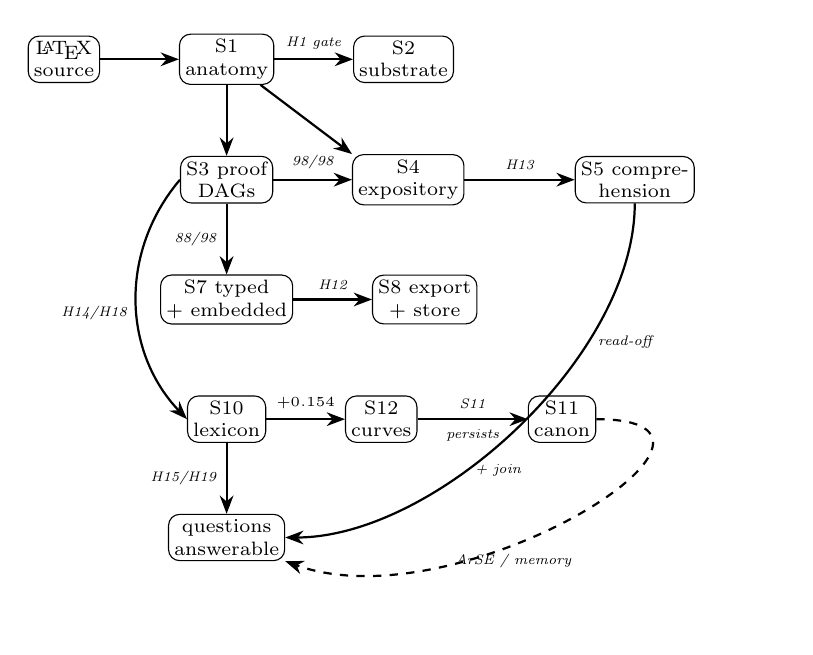
\begin{tikzpicture}[
  every node/.style={font=\scriptsize},
  var/.style={draw, rounded corners, minimum height=5.5mm, inner sep=2pt, align=center},
  wk/.style={draw, rounded corners, minimum height=5.5mm, inner sep=2pt, align=center, dashed},
  wit/.style={-{Stealth}, thick},
  unwit/.style={-{Stealth}, thick, dashed},
  lab/.style={font=\tiny\itshape, align=center}]

\node[var] (src) {\LaTeX\\source};
\node[var, right=10mm of src] (anat) {S1\\anatomy};
\node[var, right=10mm of anat] (sub) {S2\\substrate};
\node[var, below=9mm of anat] (iatc) {S3 proof\\DAGs};
\node[var, right=10mm of iatc] (expo) {S4\\expository};
\node[var, right=14mm of expo] (comp) {S5 compre-\\hension};
\node[var, below=9mm of iatc] (typ) {S7 typed\\+ embedded};
\node[var, right=10mm of typ] (exp) {S8 export\\+ store};
\node[var, below=9mm of typ] (lex) {S10\\lexicon};
\node[var, right=10mm of lex] (curve) {S12\\curves};
\node[var, right=14mm of curve] (canon) {S11\\canon};
\node[var, below=9mm of lex] (field) {questions\\answerable};

\draw[wit] (src) -- (anat);
\draw[wit] (anat) -- node[lab, above] {H1 gate} (sub);
\draw[wit] (anat) -- (iatc);
\draw[wit] (anat) -- (expo.north west);
\draw[wit] (iatc) -- node[lab, above] {98/98} (expo);
\draw[wit] (iatc) -- node[lab, left] {88/98} (typ);
\draw[wit] (typ) -- node[lab, above] {H12} (exp);
\draw[wit] (expo) -- node[lab, above] {H13} (comp);
\draw[wit] (iatc.west) to[bend right=42] node[lab, left, pos=0.55] {H14/H18} (lex.west);
\draw[wit] (lex) -- node[lab, above] {$+0.154$} (curve);
\draw[wit] (curve) -- node[lab, above] {S11} node[lab, below] {persists} (canon);
\draw[wit] (lex) -- node[lab, left] {H15/H19} (field);
\draw[wit] (comp.south) to[out=-90, in=0, looseness=0.8]
      node[lab, right, pos=0.3] {read-off} node[lab, right, pos=0.62] {+ join} (field.east);
\draw[unwit] (canon.east) to[out=0, in=-20, looseness=1.4]
      node[lab, below, pos=0.62] {ArSE / memory} (field.south east);
\end{tikzpicture}
\end{minipage}\hfill
\begin{minipage}[c]{0.30\textwidth}
\centering
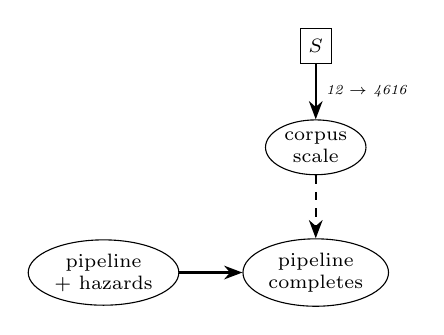
\begin{tikzpicture}[
  every node/.style={font=\scriptsize},
  var/.style={draw, ellipse, minimum height=5mm, inner sep=1.5pt, align=center},
  sel/.style={draw, rectangle, minimum height=4.5mm, inner sep=3pt},
  wit/.style={-{Stealth}, thick},
  unwit/.style={-{Stealth}, thick, dashed},
  lab/.style={font=\tiny\itshape, align=center}]
\node[sel] (S) {$S$};
\node[var, below=7mm of S] (scale) {corpus\\scale};
\node[var, below=8mm of scale] (works) {pipeline\\completes};
\node[var, left=8mm of works] (pipe) {pipeline\\+ hazards};
\draw[wit] (S) -- node[lab, right] {12 $\to$ 4616} (scale);
\draw[unwit] (scale) -- (works);
\draw[wit] (pipe) -- (works);
\end{tikzpicture}
\end{minipage}
\caption{\textbf{Left:} the mining mechanism as currently witnessed, terminating
in \emph{questions answerable} rather than in an anatomy delivered --- a
capability claim should end in what the artifacts let you ask. Solid edges carry
certificates (labels name the gate, the count, or the hazard whose repair the
edge depends on); \emph{dashed edges are what is not yet witnessed}. Two edges
that were dashed on 6 August are now solid: S5 comprehension (\hz{H13} --- its
strategy half had no producer in the DAG, and both producers turned out to
exist and be deterministic) and S11's canon (which computed a shape census and
discarded it). What remains dashed is the ArSE/memory edge: the argument graphs
carry premises, warrants and declared holes, which is the shape an adversarial
exchange or a retrieval stage needs, but nothing consumes them yet. Note that
the \emph{learning} path (S3 $\to$ S10 $\to$ S12) became solid only after
\hz{H14}, \hz{H15}, \hz{H18} and \hz{H19} were closed --- before that it either
aborted on an id, printed into a void, or measured a different corpus.
\textbf{Right:} A13 as a selection diagram. $S$ switches corpus scale (16
papers $\to$ the full field); ``the pipeline completes at field scale'' is
identified only if the $S$-dependence can be separated from the pipeline edge.
It cannot yet: \hz{H20} was a defect whose \emph{severity} is scale-dependent (a
$23\times$ waste here, ${\sim}138$k redundant rebuilds and non-termination at
field scale), which is precisely an $S$-to-outcome path that does not pass
through the pipeline edge. Scale transport is therefore a derivation
obligation, not an extrapolation --- see \S\ref{sec:prereg}.}
\label{fig:dag}
\end{figure}

``The pipeline works'' is a causal claim, and the hazards are what make it one.
Three of them are worth reading as causal structure rather than as bugs.

\hz{H19} (S10's reground scripts read hardcoded mark4-era paths) is a
\emph{confounded measurement}: the reported lift was a function of the fixture
corpus, not of the run. It failed on Zone only because a fixture paper's
source was unstaged; on a host holding all of arXiv math it would have returned
a confident number for a corpus nobody ran. The completeness ledger was built
to prevent exactly this at the \emph{stage} level after mark5, and could not
see it one level down, \emph{inside} a stage.

\hz{H20} (a missing cache, $O(\text{scope files})$ rather than
$O(\text{papers})$) is the clearest $S$-dependent hazard: harmless-looking at
$n{=}16$, fatal at $n{=}4616$. Any readiness claim that does not distinguish
scale-invariant hazards from scale-dependent ones is not a readiness claim.

\hz{H12}/\hz{H18} together say that \emph{artifact validity is
reader-relative}: a graph can pass a Clojure-side gate and be unreadable by the
Python stage that consumes it (unicode in keywords), or carry \LaTeX{} that is
not legal EDN escaping (all $42$ of S4's first-pass failures). Both were
repaired at one shared site only after being patched at two or three
independently --- the same lesson, twice, that when one reconciliation grows
several implementations the abstraction wants to be shared.

\section{The hazard ledger, in shape}
\label{sec:hazards}

Twenty-one hazards; twenty closed. Grouped by what they cost, because the groups
argue for different remedies:

\begin{center}
\small
\begin{tabular}{p{0.26\textwidth} p{0.10\textwidth} p{0.52\textwidth}}
\textbf{Class} & \textbf{Hazards} & \textbf{What the class implies}\\[2pt]
\hline\\[-8pt]
\emph{Stops the run} &
\hz{H1} \hz{H2} \hz{H3} \hz{H9} \hz{H10} \hz{H14} &
Missing commands, hardcoded model names, GPU-tuned timeouts, id parsing that
breaks one arXiv family. Loud, cheap to fix, and each would independently
have ended a cluster window.\\[3pt]
\emph{Corrupts silently} &
\hz{H12} \hz{H12b} \hz{H18} \hz{H11} \hz{H11b} &
Artifacts that pass one reader and fail the next; a server blip fast-failing a
whole batch; a region cap that misses an id family. These do not fail --- they
shrink the corpus without saying so.\\[3pt]
\emph{Destroys or misstates the findings} &
\hz{H15} \hz{H16} \hz{H17} &
The learning layer printed its results and persisted nothing; the accretion
curve wrote to a mark6-named file outside the retrieval manifest; its axis was
labelled ``papers'' while counting proof-graphs ($\approx 15\times$). The
science, not the artifacts.\\[3pt]
\emph{Measures the wrong thing} &
\hz{H19} \hz{H19b} \hz{H19c} &
Stage inputs and the measurement set defaulting to fixtures. The most dangerous
class: it neither crashes nor loses data, it returns plausible numbers.\\[3pt]
\emph{Scale-dependent} &
\hz{H20} &
Harmless at pilot size, fatal at field size. The class that a pilot cannot
detect by succeeding.\\[3pt]
\emph{Unfaithful} &
\hz{H21} &
Artifacts that do not point where they say they point. The prompt gave the
model the passage as bare text, so \texttt{:source} anchors were \emph{counted}
rather than read: $41\%$ cover the line their own text came from, median drift
$3$ lines. Content faithful, coordinates not. Found only by reading a paper
against its source (\S\ref{sec:annex}).\\[3pt]
\emph{Open} &
\hz{S11} &
One remains: the structural canon computes and discards. See \S\ref{sec:open}.\\
\hline
\end{tabular}
\end{center}

\section{Honest boundaries and the open gaps}
\label{sec:open}

\textbf{\hz{H13} --- CLOSED 7 August, and the way it closed is the point.}
It looked like the expensive gap: S5's rung-3 half reads
\texttt{data/rung3-technique/<pid>.technique.json}, and the obvious reading was
that producing it needed a mining run. It did not. Both producers already
existed and are explicitly \emph{deterministic} --- \texttt{cas\_segment.py}
turns gated graphs into proof steps, \texttt{rung3\_technique.py} turns those
into technique gap maps --- and neither appeared in any stage of the stepper.
The one real defect was a granularity mismatch: \texttt{cas\_segment} named its
output per \emph{paper} while S5 looked up per \emph{proof}, so every proof of a
paper overwrote its siblings and $98$ graphs collapsed to $12$ files, which S5
then failed to find at all. One line, plus the DAG wiring. Strategy moves went
$0 \to 202$ grounded / $564$ thin / $52$ ungrounded, and the verdict
distribution from uniformly \texttt{no-structure} to $\{$well-formed $6$,
partial $82$, weak-extraction $10\}$. Total cost: two CPU minutes.

\emph{The generalisable form:} both of this note's ``open gaps'' turned out to
be accounting rather than capability --- information the pipeline had already
computed and failed to carry across a seam. That is the same shape as
\hz{H15}/\hz{H16} (computed, printed, discarded) and \hz{H19} (computed against
the wrong inputs). It is worth asking of any remaining gap whether it is a
missing capability or a missing connection, because the second is two orders of
magnitude cheaper and, here, was the answer four times out of four.

\emph{The original diagnosis, retained:}
Comprehension is defined as R2d $\oplus$ rung-3, and the rung-3 half reads
\texttt{data/rung3-technique/<pid>.technique.json}, produced by
\texttt{rung3\_technique.py}, which appears in no stage of the stepper and no
entry of the DAG contract. The only such directory present is a mark4-era
artifact for a different corpus. Consequence, measured: all $98$ proofs score
\emph{no-structure} and \texttt{weak-proof} is unreachable. This is not a
wiring bug --- it is a choice between two repairs, and the choice changes what
a run \emph{means}: either promote \texttt{rung3\_technique} to a stage (and
trace the producers of its \texttt{--steps-dir}/\texttt{--cas-select} inputs),
or restate S5's criterion as what the pipeline can actually compute. Deferred
deliberately to the operator.

\textbf{\hz{S11} --- PARTLY CLOSED 7 August; what remains is smaller and
sharper.} The gap was that S11 computed a shape census and whole-paper
signatures and then printed both. \texttt{clean\_paper\_signature} now persists
\texttt{<run-dir>/structural-canon.json} in the shape the annex fixture
proposed: one record per shape with population and exemplars, one signature per
paper, and the paper-twin similarities ($5$ shapes, $10$ signatures, twin-sim
mean $0.75$). Learning goals \#3 and \#4 therefore survive teardown.

What is \emph{not} closed: \texttt{sfc\_struct\_canon}, which canonicalises
\emph{definition} shapes rather than proof shapes, still writes no file. Left
alone deliberately --- its natural artifact is a canonical-form table whose key
schema we have not settled, and inventing one that nothing reads would repeat
the mistake \hz{H16} punished. Unlike the original gap, this one is precisely
scoped: one script, one output, one schema decision.

\textbf{What is not claimed.} $n{=}16$ papers is a pilot; every
inductive warrant above is small. The accretion rise is \emph{recognition}
lift, not verification --- the script says so itself and we repeat it. The
mining used one model class, so A14 is registered rather than witnessed. The
XTDB bench numbers are at a corpus size where the store is not under load, and
the missing-warrant rate ($58\%$, stable from $n{=}22$ to $n{=}98$) is a
property of \emph{extraction over this literature}, not yet attributable
between literature omission and extractor failure --- that attribution is what
the three-arm exam in \texttt{E-mining-qual-loop.md} is designed to provide.

\section{What this is for}

Two things. First, it is the artifact that lets a cluster window be booked
against a tested pipeline rather than a hope: the readiness claim is now
``S1--S12 executed end-to-end, gated and ledgered, on a host nobody was
watching, with twenty-one hazards enumerated and twenty closed'', which is a
different kind of sentence from ``the stages exist''.

Second, and more transferable: the hazard ledger is a \emph{form}. The APM note
showed a capability claim decomposed into contracted holes with graded
warrants. This note adds the observation that for a pipeline, the warrants are
not enough --- because a stage can satisfy its contract while printing into a
void, or while measuring a fixture. What closes that gap is not more testing
but a different question, asked stage by stage: \emph{if this stage were
silently wrong, what would I see?} Six of the twenty-one hazards were found by
asking it, and the two open gaps are the places where the answer is still
``nothing''.

There is one further move, which \hz{H21} argues for and the annex performs:
after asking what a silent failure would look like, \emph{read one artifact
against its source}. The census counts many things approximately; a worked
example checks a few things exactly. \hz{H21} --- anchors naming the wrong line
while glossing the right text --- is invisible to every aggregate check we run,
and obvious on the first paper anyone reads.


\section{The replay harness: the ledger, made executable}
\label{sec:replay}

The slow run establishes that the stages \emph{compute}. Almost none of the
twenty-one hazards were compute failures --- they were accounting failures, and
accounting is checkable in half a second against artifacts that already exist.
So the ledger is now a regression suite: eleven checks, one per hazard class,
asserting \emph{conservation} (every proof has a steps file; every graph is
typed or logged-rejected), \emph{identity} (artifacts belong to this corpus;
metrics carry its id; both arXiv id families parse), \emph{shape} (graphs load
through the \emph{consuming} reader; refs resolve; anchors sit inside their
passage), and \emph{persistence} (the run directory holds what RETRIEVE
promises; twelve stages ledgered; the curve rises).

Each check declares the earliest stage at which it is meaningful, which turns
the suite into a \textbf{mid-run abort gate}. At \texttt{-{}-through S3} seven of
the eleven apply and four are deferred; the seven include every check that
catches a catastrophic hazard. That matters operationally: a cluster window is
booked in one large block, but a run producing artifacts that violate these
invariants will not repair itself downstream, so the honest move on a failed
prefix is to abort and give the remaining hours back. Three severities keep the
gate actionable --- \textsc{fail} (artifacts violate an invariant: abort),
\textsc{warn} (provenance imperfect, artifacts sound: continue), and
not-yet-applicable. Provenance noise must never be a reason to abandon a
window; artifact corruption must always be.

Its first run found two defects, one of them \emph{ours}: $58$ of the $98$
graphs came from four papers outside the declared manifest --- leftovers from
the top-100 shard run in a shared output directory, which every downstream stage
was then pointed at. Every corpus-level number in this note is therefore over a
sixteen-paper mixture, and said so only after a harness we wrote to catch
corpus-identity errors caught ours. The stage-mechanics claims are unaffected;
the corpus label was corrected rather than the artifacts discarded.

% "16 papers by the numbers" + query catalogue — \input{} from capability-proof-arxiv.tex
\section{Sixteen papers, by the numbers}
\label{sec:numbers}

Figure~\ref{fig:dag}'s edges say \emph{that} each stage delivers. This section
says \emph{how much}, because a witness with no weight behind it is an anecdote.
All counts are over \texttt{math-ct-e2e-16}, re-derived from the artifacts
rather than lifted from the logs that produced them, and independently
reproduced by a second reviewer. Reproducing them requires filtering to the
frozen 16-id manifest: the census script scans a mutable output directory by
default, which is the same corpus-identity hazard the harness checks for
(\S\ref{sec:replay}).

\begin{center}
\small
\begin{tabular}{p{0.20\textwidth} r p{0.52\textwidth}}
\textbf{Stage / witness} & \textbf{count} & \textbf{composition}\\
\hline\\[-8pt]
S1 marks & \textbf{320{,}337} &
over $16/16$ papers. \emph{classified} $89{,}348$ · \emph{symbol-grounded}
$68{,}484$ · \emph{math} $50{,}607$ · \emph{concept} $46{,}001$ · \emph{symbol}
$12{,}499$\\[3pt]
S1 variable grounding & \textbf{7{,}795} &
\texttt{bind/typed} marks --- variables bound to a type. Plus
\texttt{constrain/relation} $6{,}758$, \texttt{let-binder} $4{,}465$,
\texttt{definiendum} $4{,}466$\\[3pt]
S3 argument graphs & \textbf{98} &
$883$ nodes ($719$ claim, $145$ object, $19$ ref) and $419$ typed inference
edges\\[3pt]
S3 relation grammar & \textbf{62 types} &
heavy-headed: \emph{because} $161$, \emph{implies} $69$, \emph{therefore} $30$,
\emph{follows-from} $23$, then a long singleton tail\\[3pt]
S3 warrants & \textbf{383} &
\emph{missing-warrant} $222$ ($58\%$) · \emph{claim} $108$ · \emph{citation}
$53$. Each missing warrant \emph{names} the elided step\\[3pt]
S3 declared holes & \textbf{410} &
mirrored into the top-level \texttt{:holes} vector, which is what the gate
checks\\[3pt]
S4 expository scopes & \textbf{280} &
across \textbf{20 distinct scope kinds}: \emph{connection/example-source} $112$
· \emph{connection/literature-gap} $39$ · \emph{auxiliary-construction} $24$ ·
\emph{connection/transfer} $15$ · \emph{universal-property/characterizes} $13$ ·
\emph{difficulty-assessment} $8$\\[3pt]
S4 filled slots & \textbf{222} &
typed: \emph{example} $83$ · \emph{other-structure} $34$ ·
\emph{prior-result} $22$ · \emph{auxiliary} $13$ ·
\emph{characterizing-property} $11$ ($163$ total); plus $59$ carrying the
generic \texttt{slot} key\\[3pt]
S7 typed boxes & \textbf{358} &
over $88$ typed proofs, in $8$ methods: \emph{reduce-to-known-result} $204$ ·
\emph{construct-auxiliary-object} $100$ · \emph{transport-along-symmetry} $16$ ·
\emph{quotient-by-irrelevance} $13$ · \emph{compute-invariant} $11$ ·
\emph{local-to-global} $7$ · \emph{argue-by-contradiction} $4$ ·
\emph{count-by-decomposition} $1$\\[3pt]
S7 sorry-holes carried & \textbf{198} &
IATC holes converted into discharge obligations in the APM vocabulary\\[3pt]
S5 strategy moves & \textbf{818} &
$202$ grounded · $564$ thin · $52$ ungrounded. Verdicts: well-formed $6$,
partial-comprehension $82$, weak-extraction $10$\\[3pt]
S10 move lexicon & \textbf{732} &
distinct entries over $737$ moves; mean anchor confidence $0.43$ ($197$ high,
$298$ low)\\[3pt]
S11 canon & \textbf{5 shapes} &
$9$ paper signatures (papers with $\ge 2$ proofs); and $97$ definitions
reducing to $77$ canonical shapes with no coverage gaps\\[3pt]
S12 curve & \textbf{9 checkpoints} &
proof-move grounding $0.118 \to 0.272$, rising\\
\hline
\end{tabular}
\end{center}

Three of these carry more than their size suggests. The \textbf{S7 method
distribution} is the archetype census in miniature and is strikingly top-heavy:
$85\%$ of typed boxes fall into one of two methods. The \textbf{$58\%$
missing-warrant rate} holds from $n{=}22$ to $n{=}98$ and is the quantified form
of the Lakatos observation --- published mathematics deletes its scaffolding,
and the IATC layer's task is to record the deletion rather than repair it. And
\textbf{$97$ definitions reducing to $77$ shapes} is a compression ratio of
only $1.26\times$: at this corpus size definitions almost never repeat
structurally. Whether that ratio climbs with scale is the sharpest test of the
structural-canon idea (\S\ref{sec:prereg}).

\section{What can be asked of it}
\label{sec:queries}

A capability proof should terminate in questions answerable, not in an anatomy
delivered. The following are grouped by what answering them costs, which is the
distinction that matters operationally: a \emph{read-off} needs one query
against the store; a \emph{light inference} needs a join or a traversal; the
third requires machinery not yet connected, and is listed to mark the boundary
rather than to elide it.

\paragraph{Read-off (one query against the store).}
\begin{itemize}
\item \emph{Which proofs in this corpus reduce to a known result rather than
construct anything?} --- $204$ boxes, by method.
\item \emph{What did this paper's author consider too obvious to justify?} ---
the $222$ missing-warrants, each naming its elided step, filtered by paper.
\item \emph{Where does the literature say it has a gap?} ---
$39$ \texttt{connection/literature-gap} scopes.
\item \emph{Which results are cited rather than proved here?} --- $53$
\texttt{:citation} warrants with their targets.
\item \emph{What examples does the field reach for when motivating a
definition?} --- $83$ filled \texttt{:example} slots.
\item \emph{Show me every claim anchored to lines 170--180 of this paper} ---
the standoff anchors, which is the annex's own query.
\end{itemize}

\paragraph{Light inference (a join or a traversal).}
\begin{itemize}
\item \emph{Which two papers argue most alike despite being on different
topics?} --- nearest neighbour over the S11 structural signatures.
\item \emph{Which elided justifications recur across papers?} --- group
\texttt{:wanted} keys across the $410$ holes; a recurring hole is a candidate
lemma the field keeps assuming.
\item \emph{What is this proof's shape, as a sequence?} --- the
\texttt{:clean/seq} macro sequence, e.g.
\texttt{[:construct-auxiliary-object :reduce-to-known-result]}.
\item \emph{Which proofs are structurally nearest to this one?} --- the
structure embedding, off-diagonal cosine $0.02$, so neighbours are meaningful.
\item \emph{Which concepts are used but never defined in the corpus?} ---
S2 substrate minus S1 \texttt{definiendum} marks.
\item \emph{Does this paper's rhetoric match its mathematics?} --- join S4
scope kinds against S7 methods per paper; a paper full of
\texttt{difficulty-assessment} whose proofs are all
\texttt{reduce-to-known-result} is saying one thing and doing another.
\end{itemize}

\paragraph{Needs machinery not yet connected (named, not claimed).}
\begin{itemize}
\item \emph{Has this argument been made before, anywhere in the field?} ---
needs the full corpus; over a sample the negative answer is worthless
(\S\ref{sec:prereg}).
\item \emph{Retrieve the memory most relevant to this proof obligation} ---
needs the extraction wired to the memory system's retrieval stage; the
store currently has index-reach and not the affordances retrieval expects.
\item \emph{Is this sorry dischargeable from what the corpus already knows?}
--- needs the S7 \texttt{:sorry} vocabulary joined to the APM formalisation
ledger. The vocabularies already match, which is why this is a connection
rather than a capability.
\item \emph{Argue with it} --- ArSE-style adversarial exchange over a mined
argument graph. The graph carries premises, warrants and declared holes, which
is the shape such an exchange needs, but nothing consumes it yet.
\end{itemize}

Each item in the third list is a \emph{connection} between components that
exist rather than a capability that is absent --- the same distinction that
governs four of the six gaps in \S\ref{sec:open}. It is a claim the next run
should be designed to falsify, since the one counterexample there
(\hz{H22}, a missing host dependency) shows the distinction is a useful prior
and not a law.


% Preregistration section for capability-proof-arxiv.tex — included via \input{}.
\section{Preregistration: what scale is supposed to buy}
\label{sec:prereg}

The operator's reading, which this section takes as its null hypothesis: 4{,}616
\texttt{math.CT} papers differ from our 16 \emph{in scale, not in kind}, and
500{,}000 arXiv papers differ again in scale only --- so the effect of scale is
to put a $\forall$ in front of propositions that currently carry an $\exists$.
That is mostly right, and where it is right, preregistration is close to
vacuous: nobody learns anything from predicting that a stage which typed 88
graphs will type 8{,}800.

It is worth separating the propositions by what scale actually does to them,
because only one of the three classes is a real bet.

\paragraph{Class A --- $\exists \to \forall$ (scale is quantifier strength).}
Coverage and capability claims: \emph{the pipeline recovers a gated argument DAG
for this proof} becomes \emph{\dots\ for every proof}. The mechanism is
witnessed; scale extends the domain. Nothing to preregister, and the only
threat is engineering (see Class C$'$).

\paragraph{Class B --- $\forall$-shaped already; scale buys \emph{estimation}.}
Distributional facts about the field --- the missing-warrant rate, the archetype
mix, the Zipf exponent of the relation grammar. These are already universally
quantified; our 16-paper values are point estimates with wide, unstated error
bars. Scale narrows them. Preregistering an interval here is a genuine, if
modest, bet.

\paragraph{Class C --- emergent; \emph{no small-$n$ shadow at all}.}
The propositions that are not merely imprecise at $n{=}16$ but \emph{not
stateable}. Convergence is the clearest: at our scale the move lexicon holds
$732$ distinct entries over $737$ moves --- a distinct-per-move ratio of
$0.993$, i.e.\ effectively \emph{zero reuse}. ``The field's reasoning repertoire
saturates'' has no $\exists$-form to upgrade; a curve's shape is the object, and
shape needs scale. Likewise cross-paper structure (backbone saturation, variant
detection, dependency depth) does not exist in a 16-paper corpus, and retrieval
quality cannot be assessed against a store with nothing worth retrieving. This
is the class where ``scale, not kind'' might actually fail, and therefore the
only class where being wrong is informative.

\paragraph{Class C$'$ --- the engineering caveat, which we have already
falsified once.} \hz{H20} was a defect whose \emph{severity} is scale-dependent:
a $23\times$ waste at $n{=}12$, ${\sim}138$k redundant rebuilds and
non-termination at $n{=}4616$. So the pipeline at field scale is not the
pipeline at pilot scale unless the scale-dependent hazard class is empty --- and
that class is by definition the one a successful pilot cannot detect. This is
the $S$-to-outcome path in Figure~\ref{fig:dag} (right) that does not pass
through the pipeline edge.

\subsection*{Preregistered predictions}

Stated now, from the 16-paper demo, before any larger run. Each names what would
falsify it. Registered prior to any larger run.

\begin{center}
\small
\begin{tabular}{p{0.04\textwidth} p{0.42\textwidth} p{0.20\textwidth} p{0.24\textwidth}}
\textbf{\#} & \textbf{Prediction at 4{,}616 papers} & \textbf{Demo value} & \textbf{Falsified if}\\[2pt]
\hline\\[-8pt]
P1 \emph{(B)} & Missing-warrant rate on inference edges stays in $[50\%, 65\%]$ &
$58\%$, stable across $n{=}22 \to 98$ ($4.5\times$) & outside the interval\\[3pt]
P2a \emph{(C)} & The \textbf{relation grammar saturates}: fewer than $150$
distinct relation types & $62$ types, Zipf head (\emph{because} $161$,
\emph{implies} $69$) & $\ge 150$ types, or no flattening\\[3pt]
P2b \emph{(C)} & The \textbf{phrase lexicon does \emph{not} saturate}:
distinct-per-move ratio stays above $0.5$ & $0.993$ ($732/737$) & ratio falls
below $0.5$\\[3pt]
P3 \emph{(B)} & Macro archetypes stay under $15$, and
\emph{reduce-to-known} remains the plurality ($>40\%$) & $5$ macros, $67\%$
reduce-to-known & $\ge 15$ macros or plurality lost\\[3pt]
P4 \emph{(C)} & \textbf{Backbone saturation}: the citation-ranked top $10\%$ of
papers carry $\ge 50\%$ of distinct relation types & \emph{not stateable at
$n{=}16$} & top decile carries $<50\%$\\[3pt]
P5 \emph{(C$'$)} & At least one \emph{new} scale-dependent hazard appears
between $100$ and $4{,}616$ papers that the prefix gate cannot detect &
\hz{H20} was one such, found by accident & the full run is hazard-free\\[3pt]
P6 \emph{(C)} & On the three-arm exam, mined-contents (arm 1) beats raw-text
retrieval (arm 2) only \emph{above} some corpus size; at $n{\approx}16$ arm 2
ties or wins & \emph{not yet run} & arm 1 wins at $n{=}16$, or never wins\\
\hline
\end{tabular}
\end{center}

\medskip
\textbf{P2a/P2b are the pair worth the ink}, because together they are a claim
about what the lexicon \emph{is}. Our harvest currently records instantiated
claims (``$l$ is an exact localization functor''), not abstract move types ---
which is why its reuse is nil. The relation grammar is the move-\emph{type}
layer, and it is small and heavy-headed. If P2a and P2b both hold, ``the field's
reasoning repertoire'' is the grammar, the phrase lexicon is an index rather
than a vocabulary, and the S10 metric should be re-read accordingly. If P2b
fails --- if phrases do start repeating at scale --- then mathematical prose is
more formulaic than we think, which would be the more interesting result.

\textbf{P5 is the prediction we would bet on hardest}, and it is the one that
makes the operator's null hypothesis conditional rather than free: ``scale, not
kind'' holds for the \emph{claims} and fails intermittently for the
\emph{machinery}. That is precisely why the abort gate exists at a prefix, and
why it cannot be trusted to catch everything.

\subsection*{What ``complete'' might change, if anything}

One residual possibility deserves naming rather than dismissing. A
\emph{complete} field --- every \texttt{math.CT} paper, not a sample --- admits
questions a sample cannot answer even in principle: whether a given argument
pattern is \emph{unique} to a paper, whether a definition has a first
occurrence, whether a proof technique is \emph{absent} from a subfield. These
are $\neg\exists$ claims, and negative existentials over a sample are worthless
while over a complete corpus they are evidence. If scale changes kind anywhere,
it is here: not in what the pipeline extracts, but in which questions the
extraction can be asked.


% Annex to capability-proof-arxiv.tex — included via \input{}.
\appendix
\section{Annex: one paper, end to end}
\label{sec:annex}

The warrant table asserts that the stages work. This annex shows one paper's
artifacts against its own source, so the assertion can be checked rather than
believed. The paper is \texttt{arXiv:2311.05789}, chosen because it is small
enough to display whole and complete across every layer: 2 proof passages, 2
CLean typings, 6 expository scopes. Nothing here is reformatted for
presentation --- the EDN is as the pipeline emitted it, and the source lines
are as \texttt{dp\_paper\_view} numbers them.

\subsection*{A.1 The source, with what each stage took from it}

\begin{center}
\small
\begin{tabular}{r|p{0.52\textwidth}|p{0.29\textwidth}}
\textbf{line} & \textbf{source (\LaTeX, truncated)} & \textbf{stage annotation}\\
\hline
\multicolumn{3}{l}{\emph{\quad Introduction --- expository region, S4 window L102--120}}\\
\hline
104 & \texttt{Monoidal categories were defined in \textbackslash cite\{be\} and further studied in \dots} & S1 citation marks\\
112 & \texttt{The concept of \{\textbackslash em fusion\} \dots\ originated in high energy physics} & \\
114 & \texttt{Currently the largest consumer of fusion categories is condensed matter physics (topological states of matter)} & \textbf{S4} $\to$ \texttt{:connection/}\linebreak\texttt{application-domain}\\
\hline
\multicolumn{3}{l}{\emph{\quad Definitions --- proof passage \texttt{p0}, S3 window L170--180}}\\
\hline
174 & \texttt{commutes for any \$X,Y\textbackslash in\textbackslash C\$.} & \\
176 & \texttt{Clearly composites of semi-groupal functors and natural transformations are semi-groupal.} & \textbf{S3} node \texttt{:semi-groupal-}\linebreak\texttt{composition} (\emph{anchored} \texttt{171--172}; \textbf{H21})\\
179 & \texttt{A semi-groupal category \$\textbackslash C\$ is \{\textbackslash em monoidal\} if it has an object \$I\textbackslash in\textbackslash C\$ \dots} & \textbf{S3} node \texttt{:monoidal-}\linebreak\texttt{category-def} (\emph{anchored} \texttt{173--180})\\
180 & \texttt{\textbackslash beq\textbackslash lb\{uc\}\textbackslash xygraph\{} & \textbf{S3} node \texttt{:unit-}\linebreak\texttt{coherence-diagram}\\
\hline
\multicolumn{3}{l}{\emph{\quad Module categories --- proof passage \texttt{p1}, S3 window L307--331}}\\
\hline
307 & \texttt{A \{\textbackslash em pivotal structure\} on a rigid monoidal \$\textbackslash C\$ is a monoidal isomorphism \$\textbackslash tau\$ \dots} & \textbf{S3} \texttt{:pivotal-def} \emph{(307--307 --- exact)}\\
308 & \texttt{The group \$Aut\_\textbackslash ot(Id\_\textbackslash C)\$ acts freely on the set of pivotal structures \dots} & \textbf{S3} \texttt{:aut-action} \emph{(308--308 --- exact)}\\
310 & \texttt{For an endomorphism \$f:X\textbackslash to X\$ \dots\ \$tr(f)=ev\_\{X\^{}*\}(\textbackslash tau\_X f\textbackslash ot 1)coev\_X\$} & \textbf{S3} \texttt{:trace-def} \emph{(310--310 --- exact)}\\
311 & \texttt{A pivotal category \$\textbackslash C\$ is \{\textbackslash em spherical\} if \$tr(f\^{}*) = tr(f)\$ \dots} & \textbf{S3} \texttt{:spherical-def} \emph{(311--311 --- exact)}\\
319 & \texttt{A category \$\textbackslash M\$ is a \{\textbackslash em (left) module\} category over \$\textbackslash C\$ \dots} & \textbf{S3} \texttt{:module-}\linebreak\texttt{category-def} \emph{(exact)}\\
325 & \texttt{A natural transformation \$c:F\textbackslash to G\$ between \$\textbackslash C\$-module functors \dots} & \textbf{S3} \texttt{:module-natural-}\linebreak\texttt{trans} \emph{(anchored 327 --- off by 2)}\\
\hline
\end{tabular}
\end{center}

Read the third column as the pipeline's own claim about the second. The
\emph{content} is faithful throughout: every node text is a recognisable gloss
of the line it names, and none is invented. The \emph{anchors} are exact for
five of six nodes in \texttt{p1} and drift four to five lines in \texttt{p0} ---
which is \hz{H21}, visible here in a way no aggregate count reached, and the
reason this annex exists.

\subsection*{A.2 What S3 produced (verbatim, passage \texttt{p0})}

\begin{center}\small
\begin{minipage}{0.93\textwidth}\ttfamily\raggedright\footnotesize
\{:paper/id "2311.05789", :passage/id "2311.05789:monoidal-def:170-180",\\
\ :source \{:lines [170 180], :kind :proof\},\\
\ :nodes [\{:id :semi-groupal-composition, :kind :claim,\\
\ \ \ \ \ \ \ \ \ :text "composites of semi-groupal functors and natural transformations are semi-groupal",\\
\ \ \ \ \ \ \ \ \ :source \{:lines [171 172]\}\}\\
\ \ \ \ \ \ \ \ \{:id :monoidal-category-def, :kind :claim, :text "a semi-groupal category C is monoidal if it\\
\ \ \ \ \ \ \ \ \ has a monoidal unit I and natural isomorphisms l\_X, r\_X satisfying the unit coherence condition"\dots\}\\
\ \ \ \ \ \ \ \ \{:id :unit-coherence-diagram, :kind :object, \dots\}],\\
\ :edges [\{:id :e-monoidal-def, :kind :infer, :relation :defines,\\
\ \ \ \ \ \ \ \ \ :premise :semi-groupal-composition, :conclusion :monoidal-category-def,\\
\ \ \ \ \ \ \ \ \ :warrant \{:kind :missing-warrant,\\
\ \ \ \ \ \ \ \ \ \ \ \ \ \ \ \ \ :wanted :semi-groupal-composition-is-closed-under-composition\}\}\\
\ \ \ \ \ \ \ \ \{:id :e-coherence, :relation :requires, \dots\ :wanted :naturality-and-coherence-for-monoidal-structure\}],\\
\ :holes [\{:kind :missing-warrant, :edge :e-monoidal-def, \dots\} \{\dots\}]\}
\end{minipage}
\end{center}

Two things are worth noticing, because they are the whole point of the IATC
layer. First, the edge from ``composites are semi-groupal'' to the monoidal
definition is typed \texttt{:defines} and carries an explicit
\texttt{missing-warrant} naming what the prose skipped:
\texttt{semi-groupal-} \texttt{composition-is-closed-} \texttt{under-composition}.
The word \emph{Clearly} in line 176 is exactly the deletion the warrant records.
Second, every such hole is mirrored in the top-level \texttt{:holes} vector,
which is what the gate checks; a graph asserting a hole it does not declare is
rejected.

\subsection*{A.3 What S7 made of it, and S4 beside it}

\begin{center}\small
\begin{minipage}{0.46\textwidth}\ttfamily\footnotesize\raggedright
\{:clean/proof "2311.05789\_\_p0"\\
\ :clean/typing-source :llama\\
\ :clean/seq [:construct-auxiliary-object\\
\ \ \ \ \ \ \ \ \ \ \ \ \ :reduce-to-known-result]\\
\ :clean/boxes\\
\ [\{:id :e-monoidal-def\\
\ \ \ :method :construct-auxiliary-object\\
\ \ \ :consumes [:semi-groupal-composition]\\
\ \ \ :produces :monoidal-category-def\\
\ \ \ :hole \{:kind :sorry :discharge :sorryProof\\
\ \ \ \ \ \ \ \ \ :satiety :payoff\\
\ \ \ \ \ \ \ \ \ :wanted "semi-groupal-composition-\\
\ \ \ \ \ \ \ \ \ \ \ \ \ \ \ \ is-closed-under-composition"\}\}\\
\ \ \{:id :e-coherence\\
\ \ \ :method :reduce-to-known-result \dots\}]\}
\end{minipage}\hfill
\begin{minipage}{0.46\textwidth}\ttfamily\footnotesize\raggedright
\% S4, leaf-0001 (L102--120)\\
\{:kind :connection/application-domain\\
\ :source \{:lines [102 120]\}\\
\ :slot-fill \{:application "condensed matter\\
\ \ \ physics (topological states of matter)"\}\}\\[6pt]
\% S4, leaf-0003 (L392--425)\\
\{:kind :connection/example-source\\
\ :source \{:lines [392 425]\}\\
\ :slot-fill \{:example "the category of sets,\\
\ \ \ abelian groups, and vector spaces over\\
\ \ \ a fixed field k"\}\}\\[6pt]
\% S4, leaf-0002 (L225--276)\\
\{:kind :connection\\
\ :slot-fill \{:other-structure "braided and\\
\ \ \ symmetric monoidal categories"\}\}
\end{minipage}
\end{center}

S7 types the two inference steps into the method vocabulary
(\texttt{construct-auxiliary-object} then \texttt{reduce-to-known-result}) and
carries the IATC hole through as a \texttt{:sorry} with a discharge obligation
--- which is the bridge to the APM formalisation machinery, the same
\texttt{:sorry} vocabulary on both sides. S4, working the same paper's prose
rather than its proofs, recovers what the introduction is \emph{doing}: naming
an application domain, offering an example source, connecting to a neighbouring
structure. Neither layer sees the other's spans.

\subsection*{A.4 The two open gaps, as fixtures}

The following are \textbf{illustrative fixtures, not measurements} --- they show
the shape the missing artifacts would take, so that closing \hz{H13} and
\hz{S11} is a matter of producing this rather than of deciding what to produce.

\paragraph{\hz{H13} --- what an S5 row looks like when rung-3 exists.}
Today every row reads as the left column: the strategy half is absent, so the
verdict cannot discriminate. With \texttt{rung3\_technique} promoted to a
stage, the same rows would carry the right column, and \texttt{weak-proof}
becomes reachable --- distinguishing \emph{we extracted badly} from \emph{the
proof is thin}, which is the distinction S5 exists to draw.

\begin{center}\small
\begin{tabular}{l|ccccc|l}
 & \texttt{noun} & \texttt{s:r3} & \texttt{s:pr} & \texttt{strat} & \texttt{comp} & \textbf{verdict}\\
\hline
\emph{today} (real) & 1.00 & \texttt{--} & 0.00 & 0.00 & 0.00 & \texttt{weak-extraction}\\
\emph{today} (real) & 1.00 & \texttt{--} & 0.00 & 0.00 & 0.00 & \texttt{weak-extraction}\\
\hline
\emph{fixture} & 1.00 & 0.75 & 0.40 & 0.62 & 0.81 & \texttt{comprehended}\\
\emph{fixture} & 1.00 & 0.20 & 0.10 & 0.15 & 0.34 & \texttt{weak-proof}\\
\emph{fixture} & 0.25 & 0.60 & 0.55 & 0.58 & 0.31 & \texttt{weak-extraction}\\
\end{tabular}
\end{center}

\paragraph{\hz{S11} --- what the structural canon looks like when it persists.}
S11 computes a canonical-shape census and whole-paper signatures and then
discards them. The fixture below is the artifact shape we propose:
\texttt{<run-dir>/structural-canon.json}, one record per canonical shape with
its population and exemplars, plus one signature per paper. The real S7 macro
census (5 archetypes, $67\%$ \emph{reduce-to-known}) is the evidence that a
census of this shape is computable; what is missing is only that S11 writes it.

\begin{center}\small
\begin{minipage}{0.86\textwidth}\ttfamily\footnotesize\raggedright
\{"run\_id": "mark7z", "corpus\_id": "math-ct-e2e-12",\\
\ "shapes": [\{"shape": "define-then-verify-coherence", "n": 34,\\
\ \ \ \ \ \ \ \ \ \ \ \ \ "exemplars": ["2311.05789\_\_p0", "0708.1921\_\_p2"]\},\\
\ \ \ \ \ \ \ \ \ \ \ \ \{"shape": "reduce-to-adjunction", "n": 21, "exemplars": [\dots]\}],\\
\ "signatures": [\{"paper": "2311.05789", "archetype": "definitional-survey",\\
\ \ \ \ \ \ \ \ \ \ \ \ \ \ \ "seq": [:construct-auxiliary-object :reduce-to-known-result]\}]\}
\end{minipage}
\end{center}

\subsection*{A.5 What this annex is evidence for, and what it is not}

It is evidence that the layers do what the warrant table says: S1 marks, S3
recovers a typed argument DAG with declared holes, S4 recovers rhetorical
structure from the same paper's prose, S7 types the argument into a method
vocabulary carrying the hole forward as a discharge obligation. All of it is
checkable against the source printed beside it.

It is \emph{not} evidence of corpus-scale quality: one paper, chosen for being
displayable. Its value is the opposite of the census's --- the census counts
many things approximately, the annex checks a few things exactly, and \hz{H21}
is precisely the defect that only the second can see.


\end{document}
